\documentclass[12pt]{article}

\usepackage[utf8]{inputenc}
\usepackage[T1]{fontenc}
\usepackage[polish,provide=*]{babel}
\usepackage{lmodern}
\usepackage{amsmath}
\usepackage{latexsym,amsfonts,amssymb,amsthm,amsmath}
\usepackage{enumitem}
\usepackage{hyperref}
\usepackage{float}
\usepackage{graphicx}
\usepackage{subcaption}
\usepackage{booktabs}
\graphicspath{{./images/}}

\setlength{\parindent}{0in}
\setlength{\oddsidemargin}{0in}
\setlength{\textwidth}{6.5in}
\setlength{\textheight}{8.8in}
\setlength{\topmargin}{0in}
\setlength{\headheight}{18pt}

\title{Wachadła Sprężone}
\author{Kacper Kłos}

\begin{document}

\maketitle

Abstract

\newpage
\section{Wyniki Pomiarów}

\subsection{Stałe}
Podczas raportu będziemy nadmiernie korzystać ze stałej grawitacyjnej \(g = 9{,}81 m \, s^{-2}\)

\subsection{Pomiar Statyczny}
Pomiary zaczynamy od zawieszenia sprężyny i podwieszaniu ciężarków do jej końca. 
\begin{table}[H]
    \centering
    \begin{tabular}{c|cc}
        \toprule
        \textbf{Nr} & Masa $m$ [g] & Długość sprężyny $L$ [cm] \\
        \midrule
        1  & 49{,}14  & 31{,}4 \\
        2  & 91{,}27  & 32{,}8 \\
        3  & 151{,}85 & 34{,}8 \\
        4  & 201{,}43 & 36{,}6 \\
        5  & 250{,}71 & 38{,}2 \\
        6  & 299{,}12 & 39{,}7 \\
        7  & 348{,}18 & 41{,}4 \\
        \bottomrule
    \end{tabular}
    \caption{Pomiary długości sprężyny $L$ w zależności od masy obciążenia $m$.}
    \label{tab:spring_mass}
\end{table}
Za błąd pomiarowy długości uznajemy $0{,}3 \, cm$ podczas gdy błąd wagi na poziomie $0{,}01 \, g$ uznajemy za pomijalnie mały.

Do danych jakie zebraliśmy dopasujemy parametry równania liniowego
\[
    L = a m + L_0
\]
Otrzymujemy w ten sposób wykres
\begin{figure}[H]
    \centering
    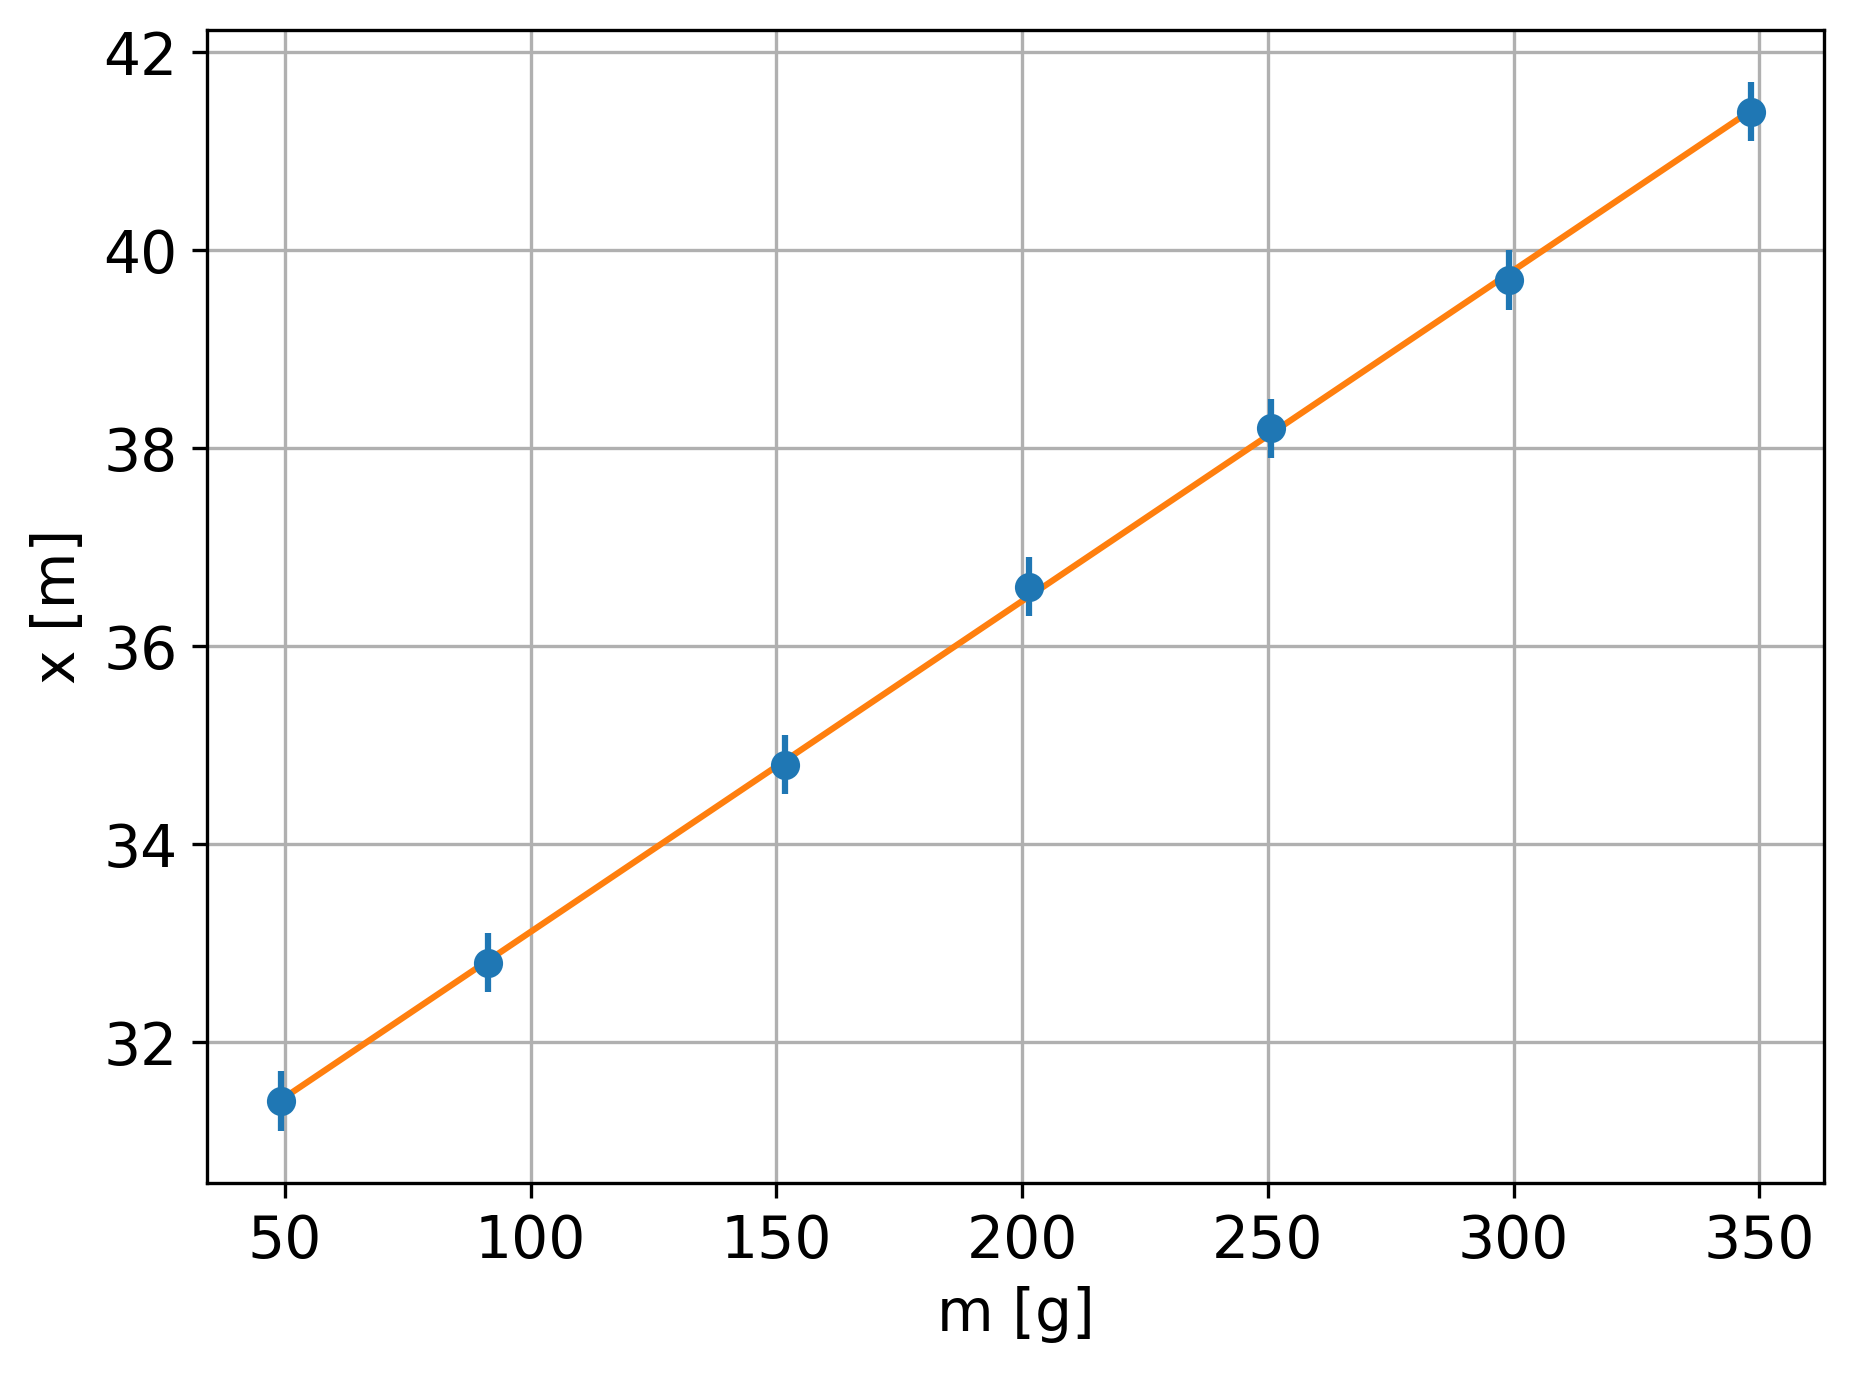
\includegraphics[width=\linewidth]{spring_mass}
    \caption{Wykres zależności długości sprężyny od zawieszonej na niej masy wraz z dopasowaniem liniowym}
    \label{fig:spring_mass}
\end{figure}
Parametry wyznaczonej krzywej wynoszą
\[
    a = (0{,}03344 \pm 0{,}00024) \, [cm \, g^{-1}], b = (29{,}77 \pm 0{,}06) \, [cm]
\]
Przy pomocy parametru a możemy wyznaczyć stałą sprężystości badanej sprężyny
\[
    k = \frac{g}{a}
\]
Co odpowiada wartości
\[
    k = (29{,}34 \pm 0{,}21) \, [m \, kg^{-1}]
\]



\subsection{Pomiar Dynamiczny}
Przy pomocy dwóch czujników PASCO PS-3219 wyznaczamy położenie obu wachadeł w zależności od czasu, zebrane dane są w pliku dołączonym do dokumentu. Zawiera on 3 serie pomiarowe po 2 pomiary, wpierw dudnienia a potem drgania w przeciwfazie dla trzech różnych odległości sprężyny od osi obrodu wachadła. Ostatnia seria zawiera pomiar dla jednego wachadła bez podłączonej sprężyny. We wszystkich poniższych pomiarach uznajemy błąd transformaty fouriera za jej rozdzielczość \(\frac{f_s}{n}\) gdzie \(f_s = 40 \, Hz\) oznacza częstotliwość pobierania danych przez detektor, a \(N\) liczbę punktów pomiarowych. Kluczowe w naszych pomiarch będzie odległość środka masy którą wyznaczyliśmy równoważąc wachadło na \(r = 79{,}7 \, cm\). Oraz istotna jest masa wachadła wynosząca \(m = (3000 \pm 40) \, g\)

\subsection{Wachadło Bez Sprężyny}

Analize danych zacznijmy od przypadku bez podłączonej sprężyny
\begin{figure}[H]
    \centering
    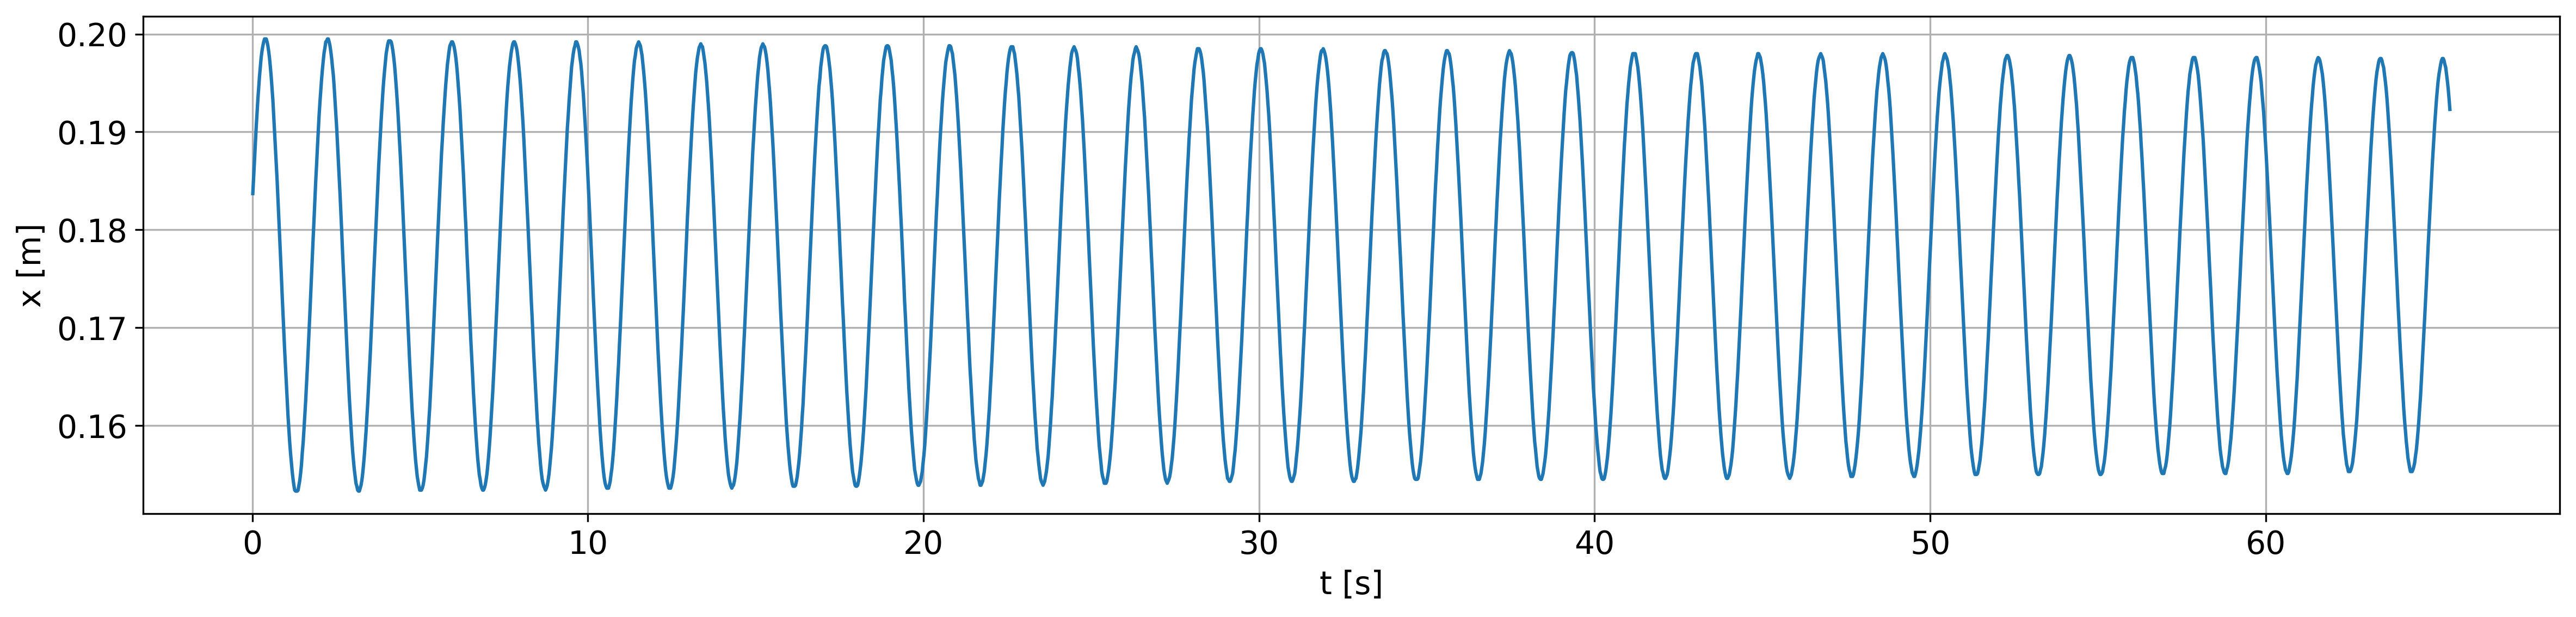
\includegraphics[width=\linewidth]{no_spring}
    \caption{Wykres zależności wychlenia od czasu dla wachadła bez sprężyny}
    \label{fig:pendulum_nospring}
\end{figure}
Aby odczytać z jaką częstotliwością drga wachadło wykonujemy transformatę Fouriera
\begin{figure}[H]
    \centering
    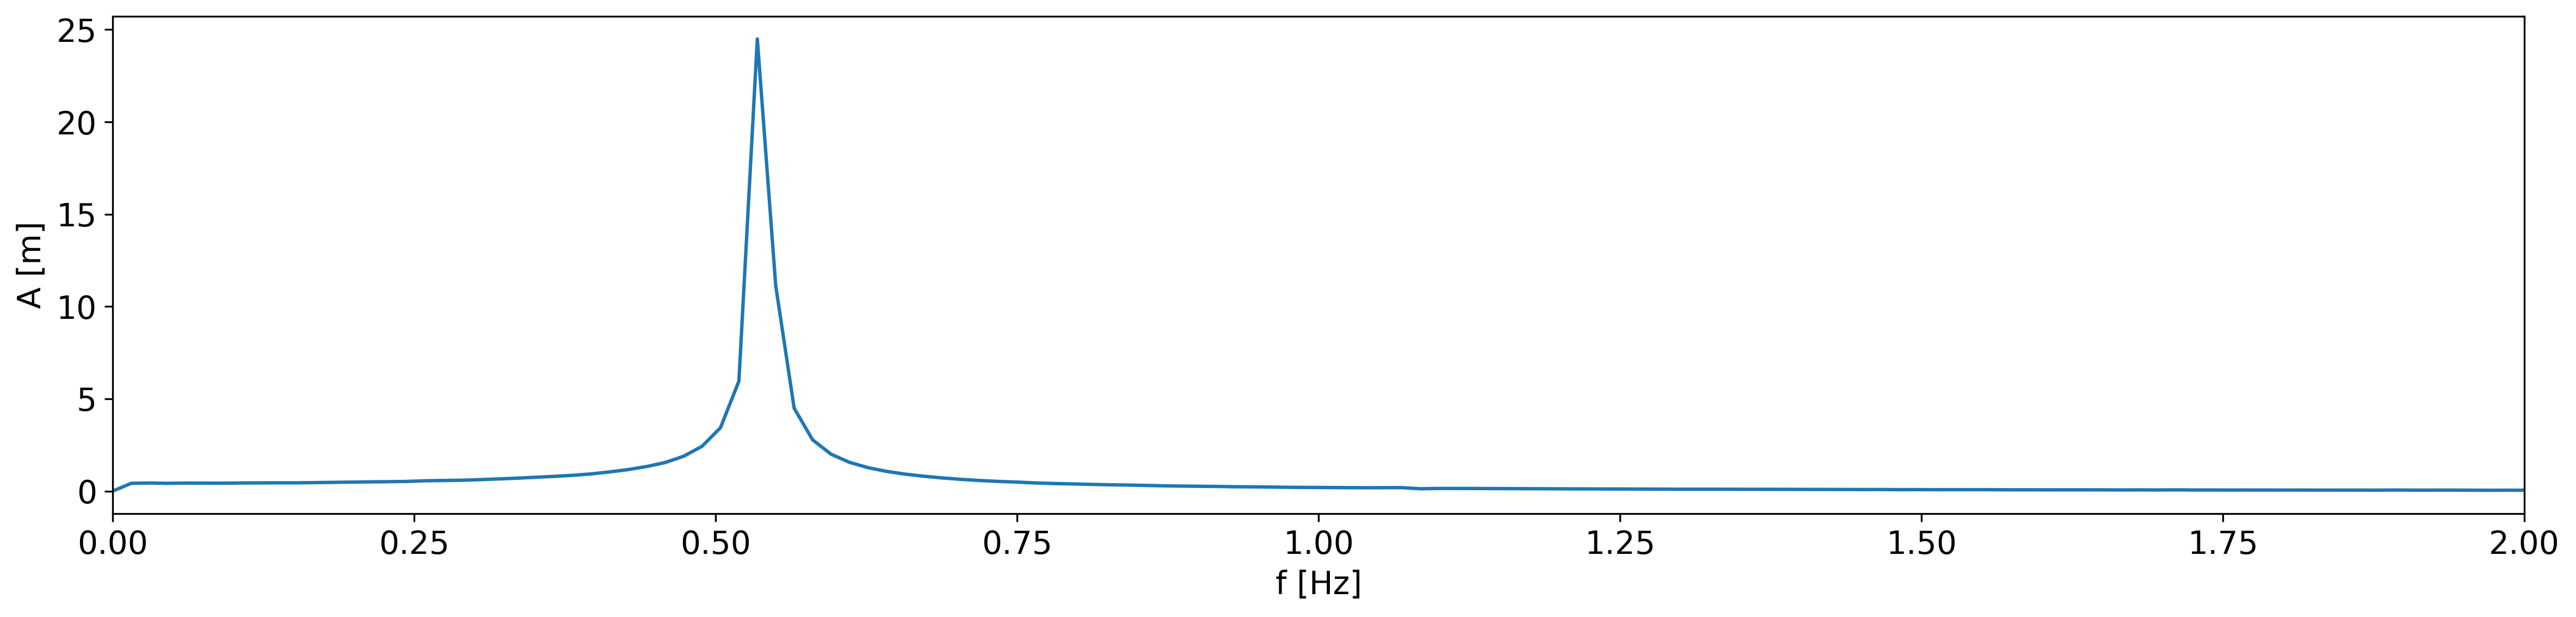
\includegraphics[width=\linewidth]{no_spring_fft}
    \caption{Wykres transformaty fouriera dla danych z wykresu \ref{fig:pendulum_nospring}}
    \label{fig:pendulum_nospring_fft}
\end{figure}
Wartość uzyskanej w ten sposób częstotliwości odpowiada
\[
    f_0 = (0{,}535 \pm 0{,}016) \, Hz
\]
Wiemy że częstotliwość drgania wachadła wynosi\cite{skrypt}
\[
    \omega_1^2 = (2\pi f_0)^2 = \frac{mgr}{I}
\]
Możemy wykorzystać ten wzór do uzyskania momentu bezwładności 
\[
    I = \frac{mgr}{(2\pi f_0)^2}
\]
\[
    I = (2{,}08 \pm 0{,}13) \, kg \, m^2
\]


\subsection{Drgania w przeciwfazie}
Przeanalizujemy zachowanie wachadeł kiedy drgają w przeciwfazie przy różnych punktach zaczepienia sprężyn, dla których wyznaczymy częstotliwość drgania przy pomocy transformaty fouriera
Wpierw analizując \(d = (30 \pm 0{,}1) cm\)
Zaczynamy od badania przeciwfazy
\begin{figure}[H]
    \centering
    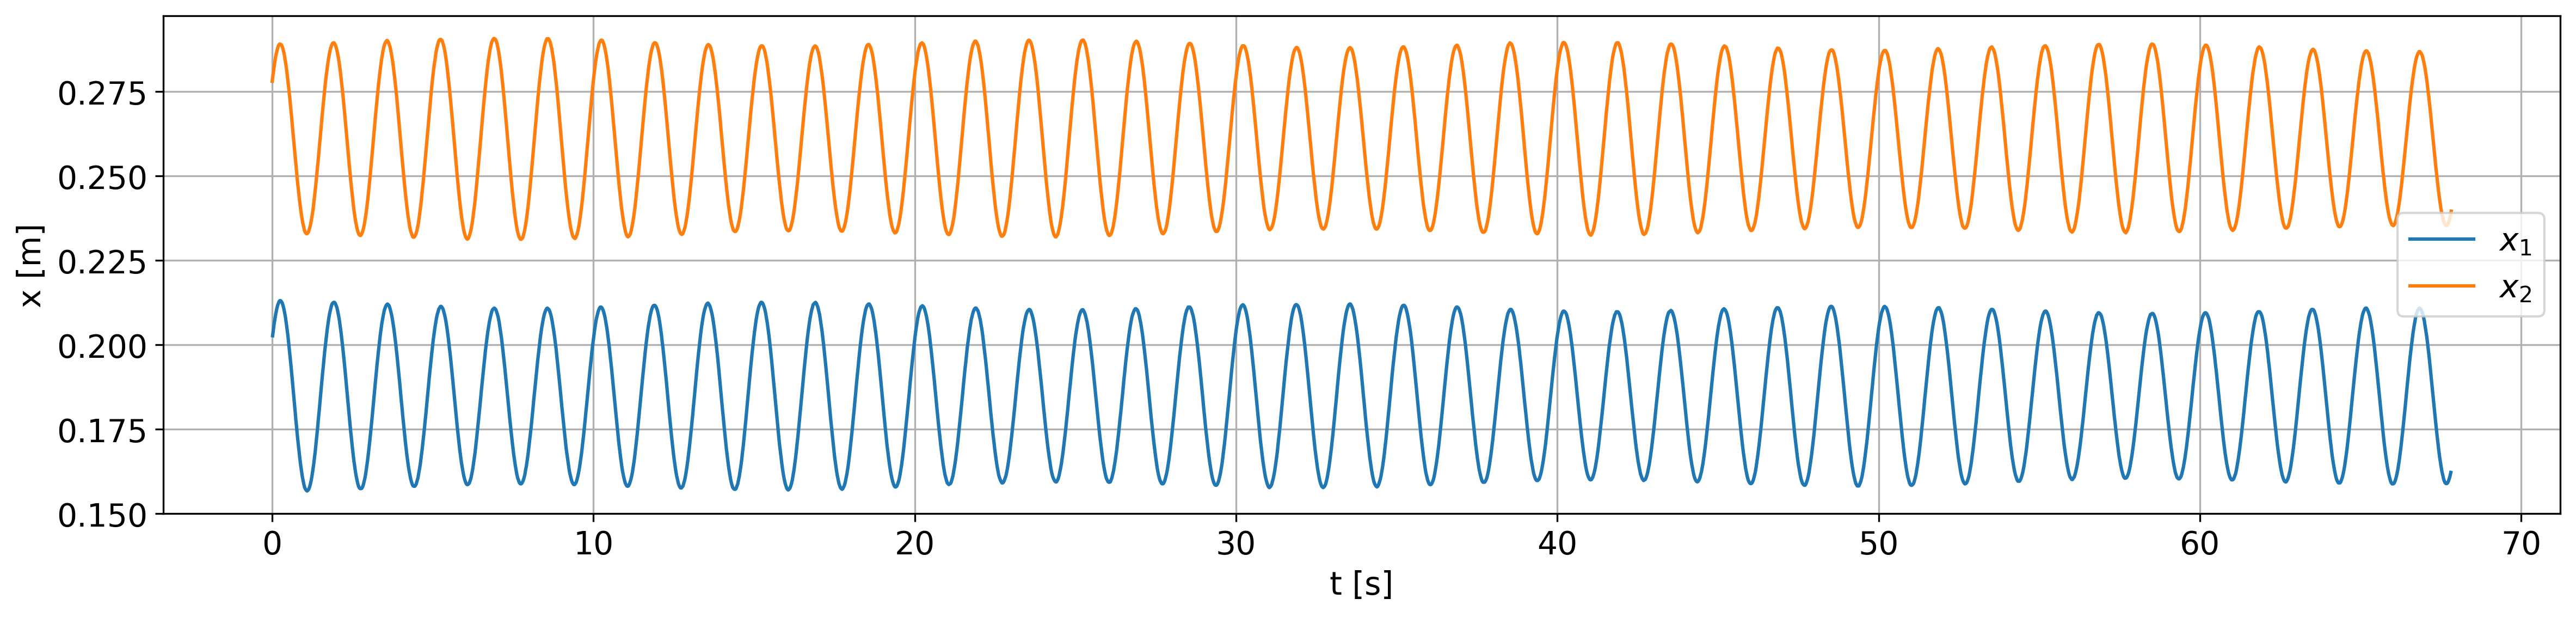
\includegraphics[width=\linewidth]{counterphase_1}
    \caption{Wykres zależności wychlenia wachadła lewego \(x_1\) i prawego \(x_2\) od czasu \(t\), dla wachadeł drgających w przeciwfazie}
    \label{fig:counter_phase_0}
\end{figure}
\begin{figure}[H]
    \centering
    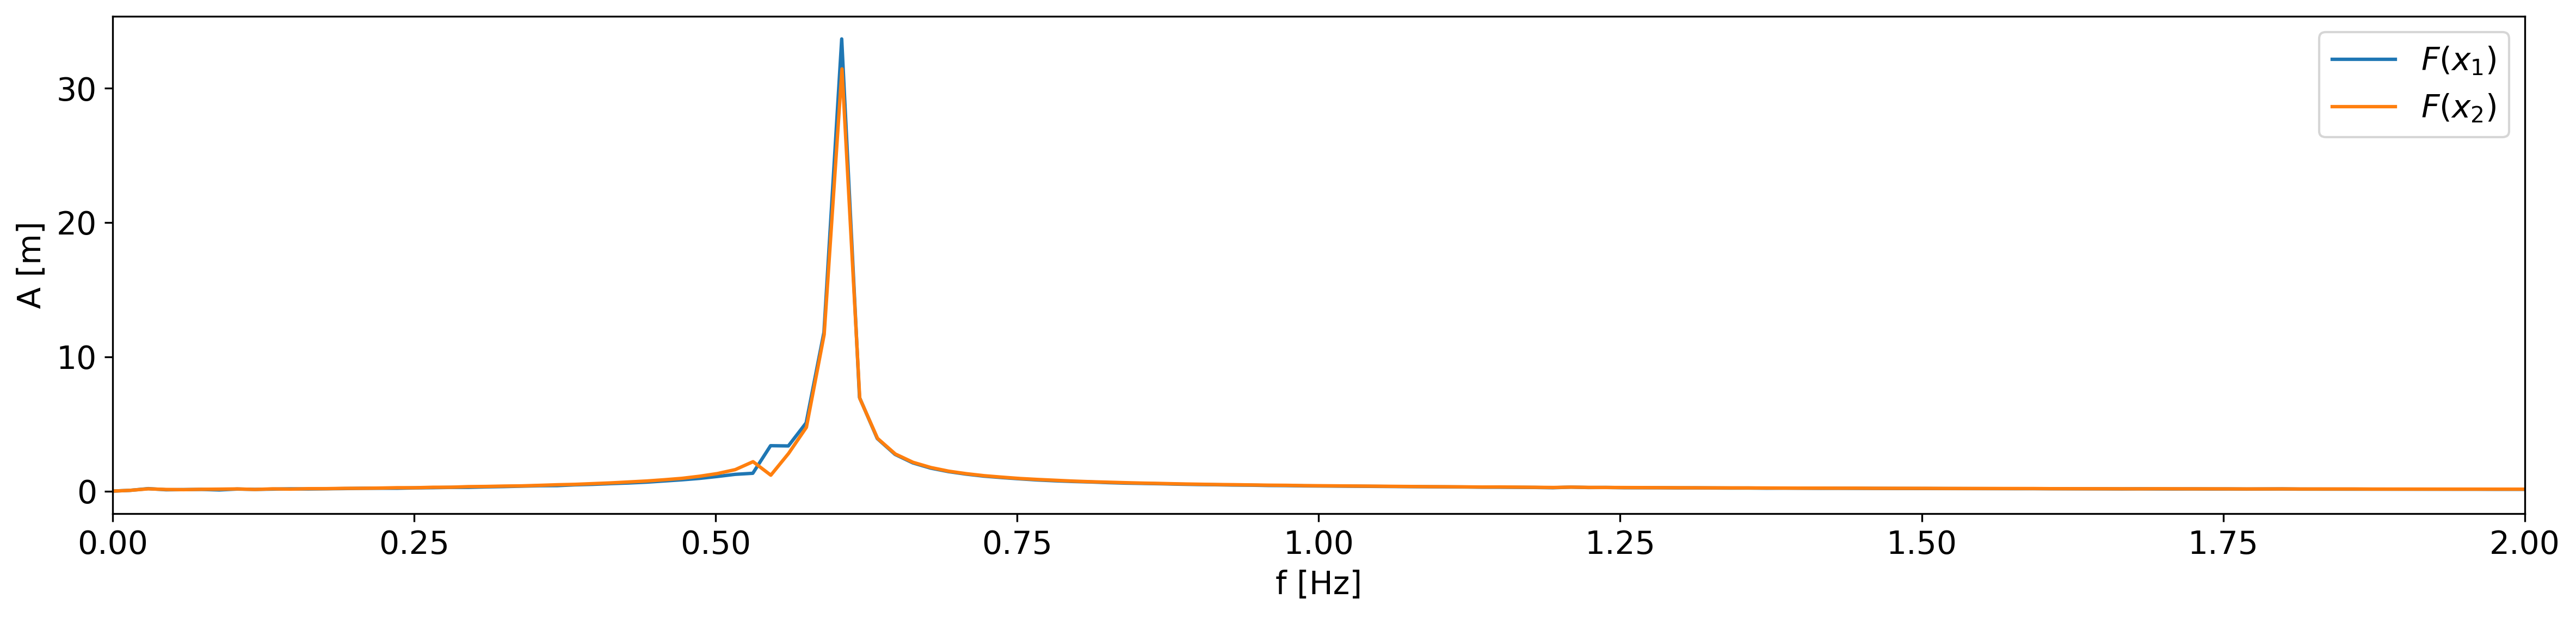
\includegraphics[width=\linewidth]{counterphase_1_fft}
    \caption{Wykres transformaty fouriera dla danych z wykresu \ref{fig:counter_phase_0}}
    \label{fig:coutner_phase_0_fft}
\end{figure}
\[
    f_{p_1} = (0{,}6045 \pm 0{,}015) \, Hz
\]
To samo wykonujemy dla \(d = (40 \pm 0{,}1) cm\)
\begin{figure}[H]
    \centering
    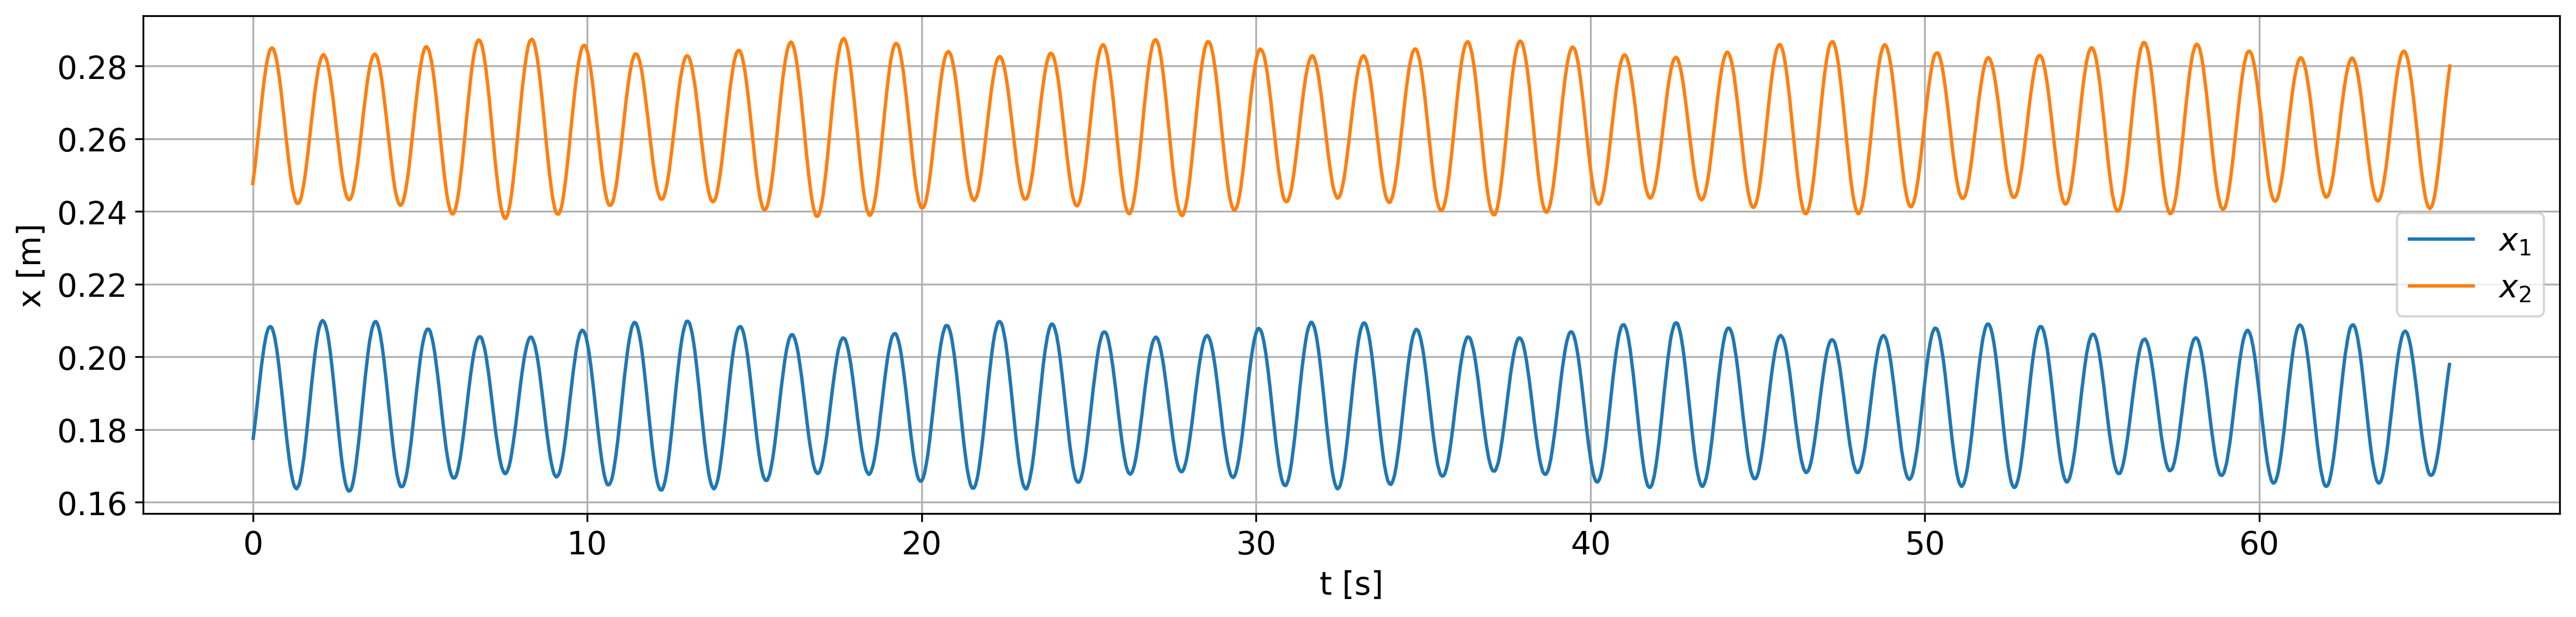
\includegraphics[width=\linewidth]{counterphase_2}
    \caption{Wykres zależności wychlenia wachadła lewego \(x_1\) i prawego \(x_2\) od czasu \(t\), dla wachadeł drgających w przeciwfazie}
    \label{fig:counter_phase_1}
\end{figure}
\begin{figure}[H]
    \centering
    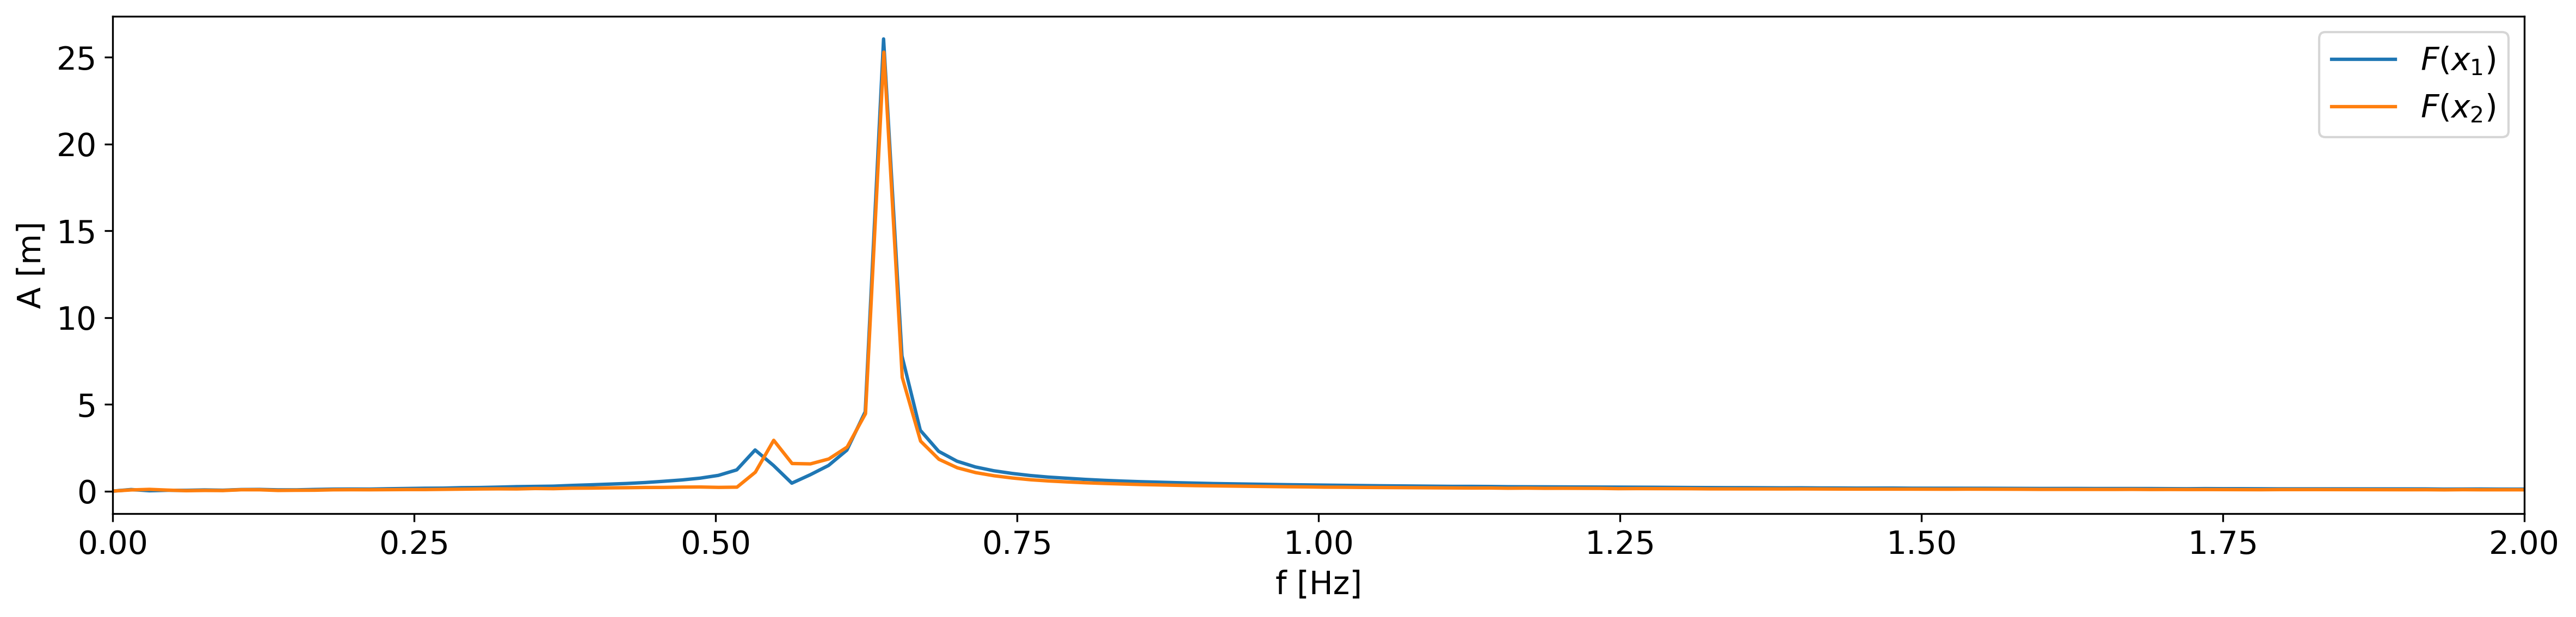
\includegraphics[width=\linewidth]{counterphase_2_fft}
    \caption{Wykres transformaty fouriera dla danych z wykresu \ref{fig:counter_phase_1}}
    \label{fig:coutner_phase_1_fft}
\end{figure}
\[
    f_{p_2} = (0{,}639 \pm 0{,}016) \, Hz
\]
Finalnie dla \(d = (45 \pm 0{,}1) cm\)
\begin{figure}[H]
    \centering
    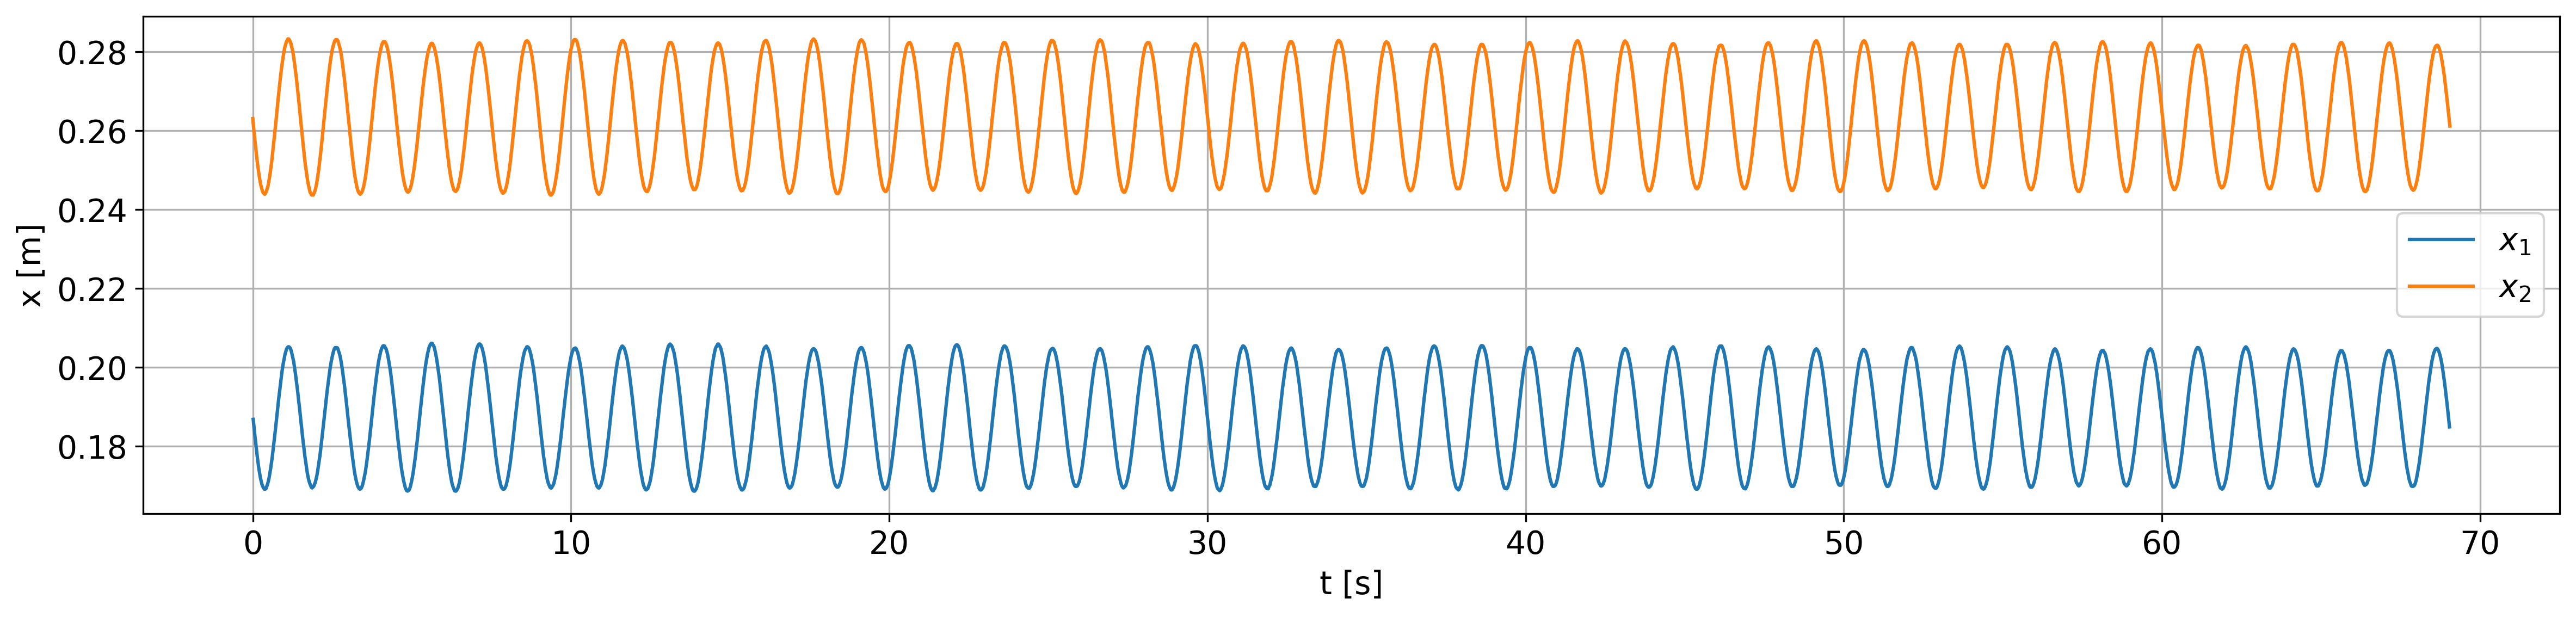
\includegraphics[width=\linewidth]{counterphase_3}
    \caption{Wykres zależności wychlenia wachadła lewego \(x_1\) i prawego \(x_2\) od czasu \(t\), dla wachadeł drgających w przeciwfazie}
    \label{fig:counter_phase_2}
\end{figure}
\begin{figure}[H]
    \centering
    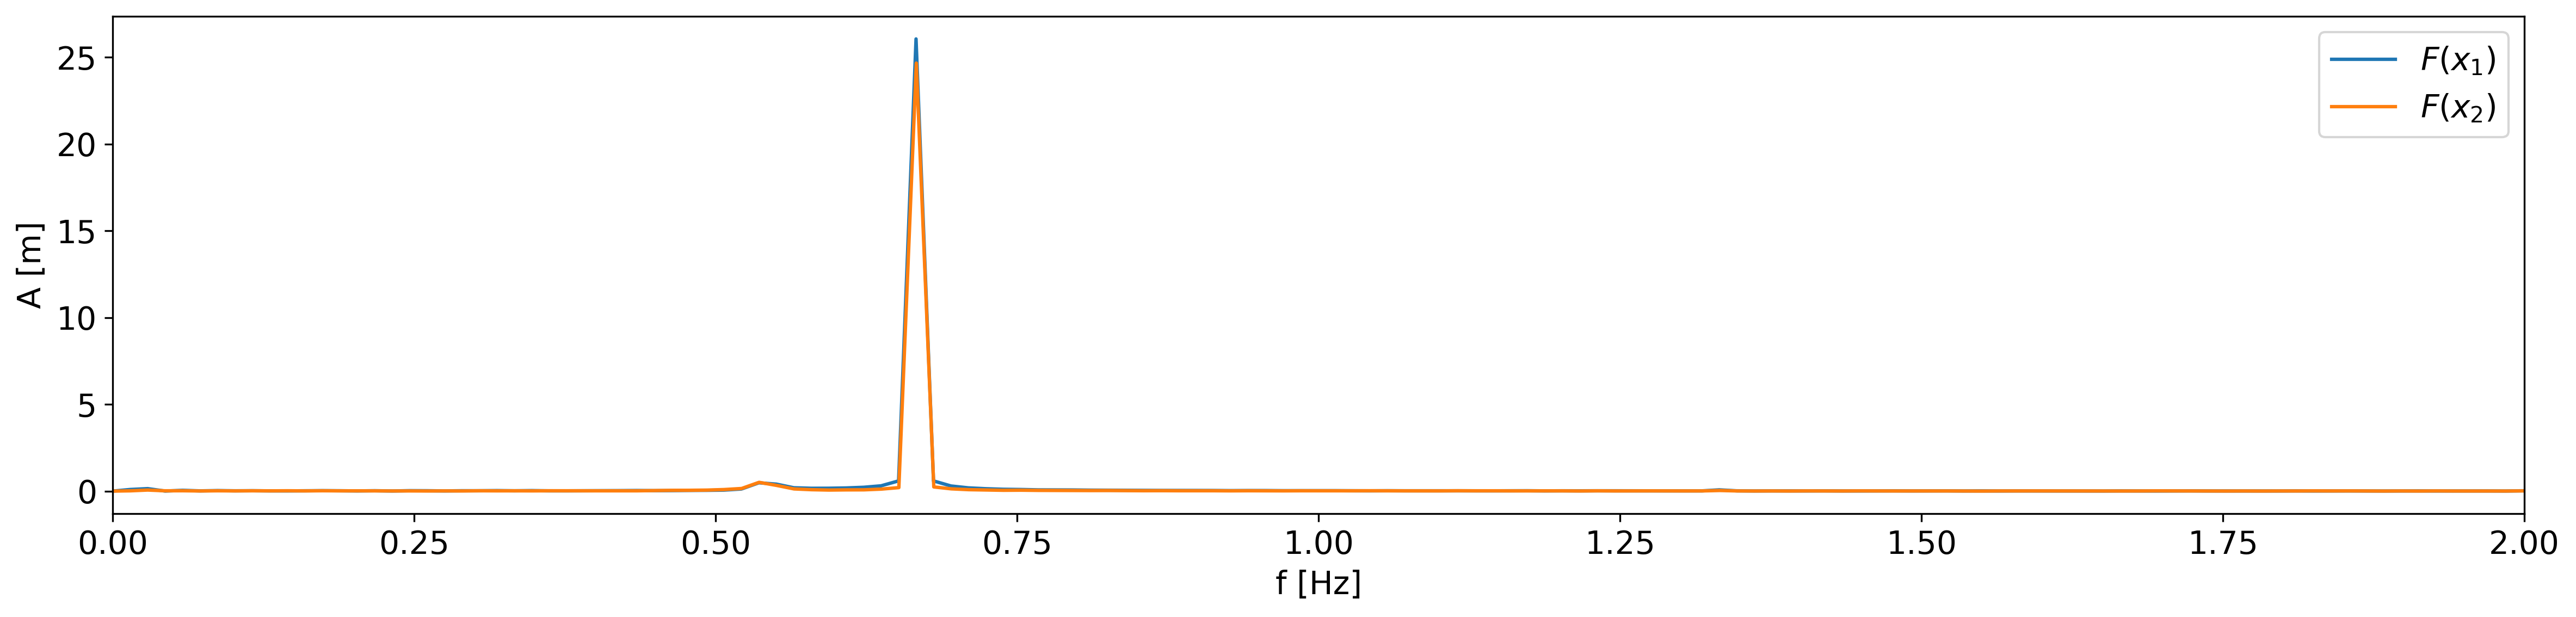
\includegraphics[width=\linewidth]{counterphase_3_fft}
    \caption{Wykres transformaty fouriera dla danych z wykresu \ref{fig:counter_phase_2}}
    \label{fig:coutner_phase_2_fft}
\end{figure}
\[
    f_{p_3} = (0{,}666 \pm 0{,}015) \, Hz
\]


\subsection{Dudnienie}
Teraz zbadamy zachowanie wachadeł podczas dudnienia i również wyznaczymy częstotliwości drgania poprzez transformatę fouriera.

Wpierw analizując \(d = (30 \pm 0{,}1) cm\)
\begin{figure}[H]
    \centering
    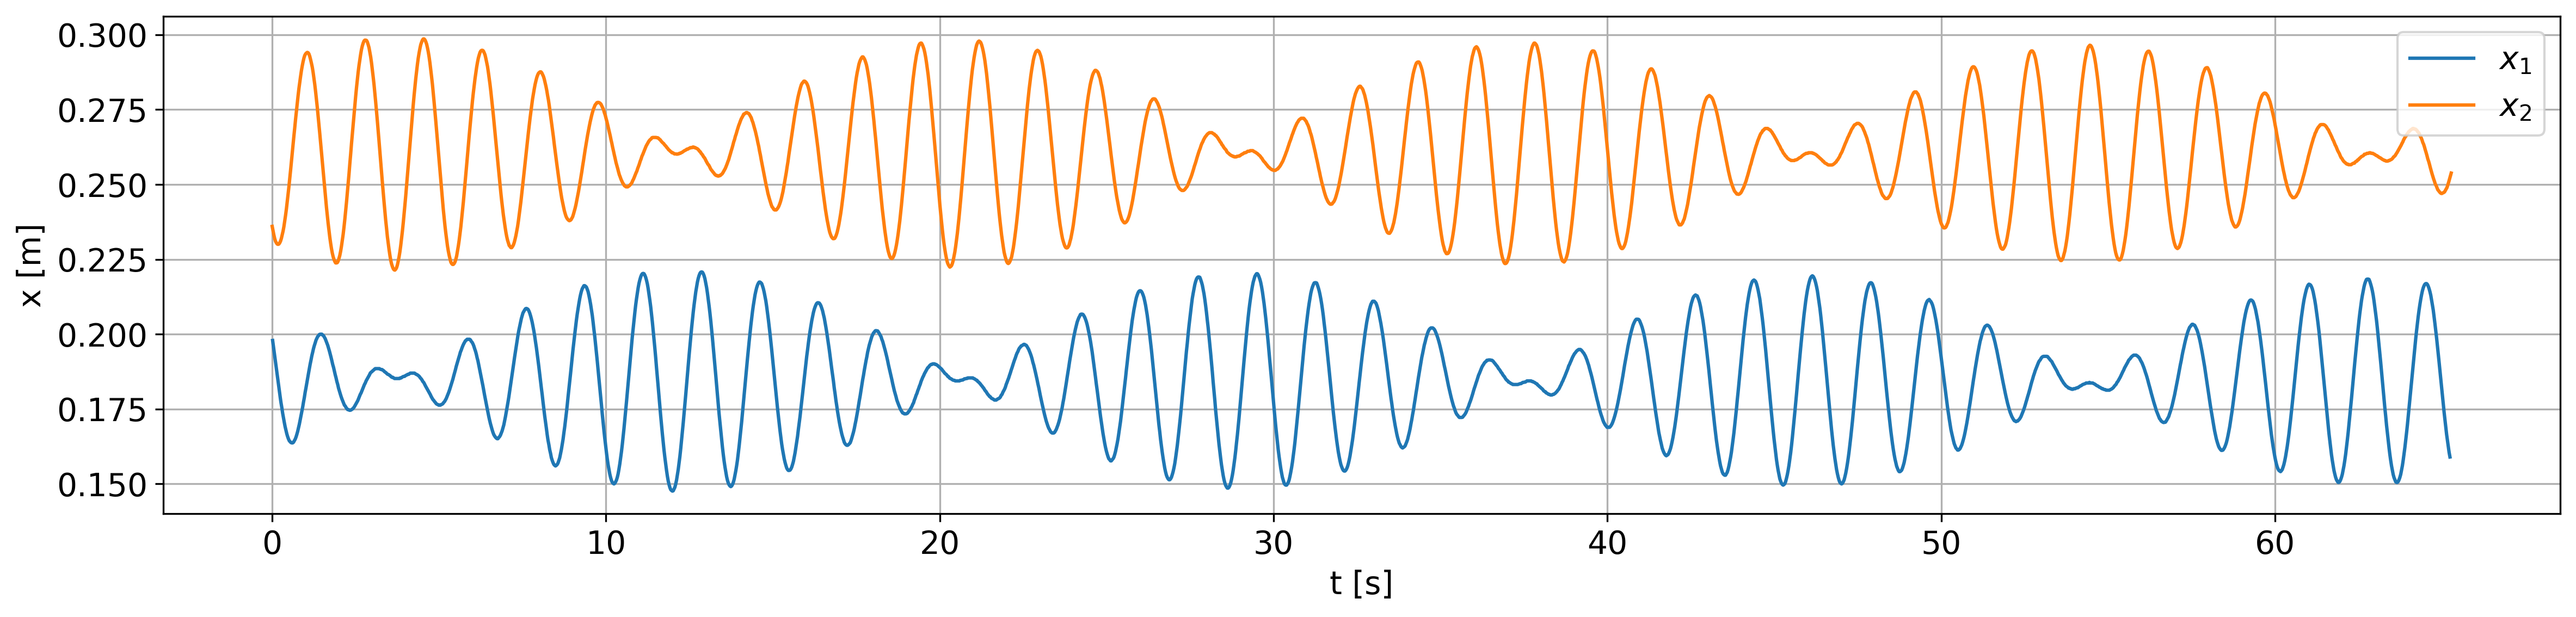
\includegraphics[width=\linewidth]{beats_1}
    \caption{Wykres zależności wychlenia wachadła lewego \(x_1\) i prawego \(x_2\) od czasu \(t\), dla wachadeł dudniących}
    \label{fig:beats_0}
\end{figure}
\begin{figure}[H]
    \centering
    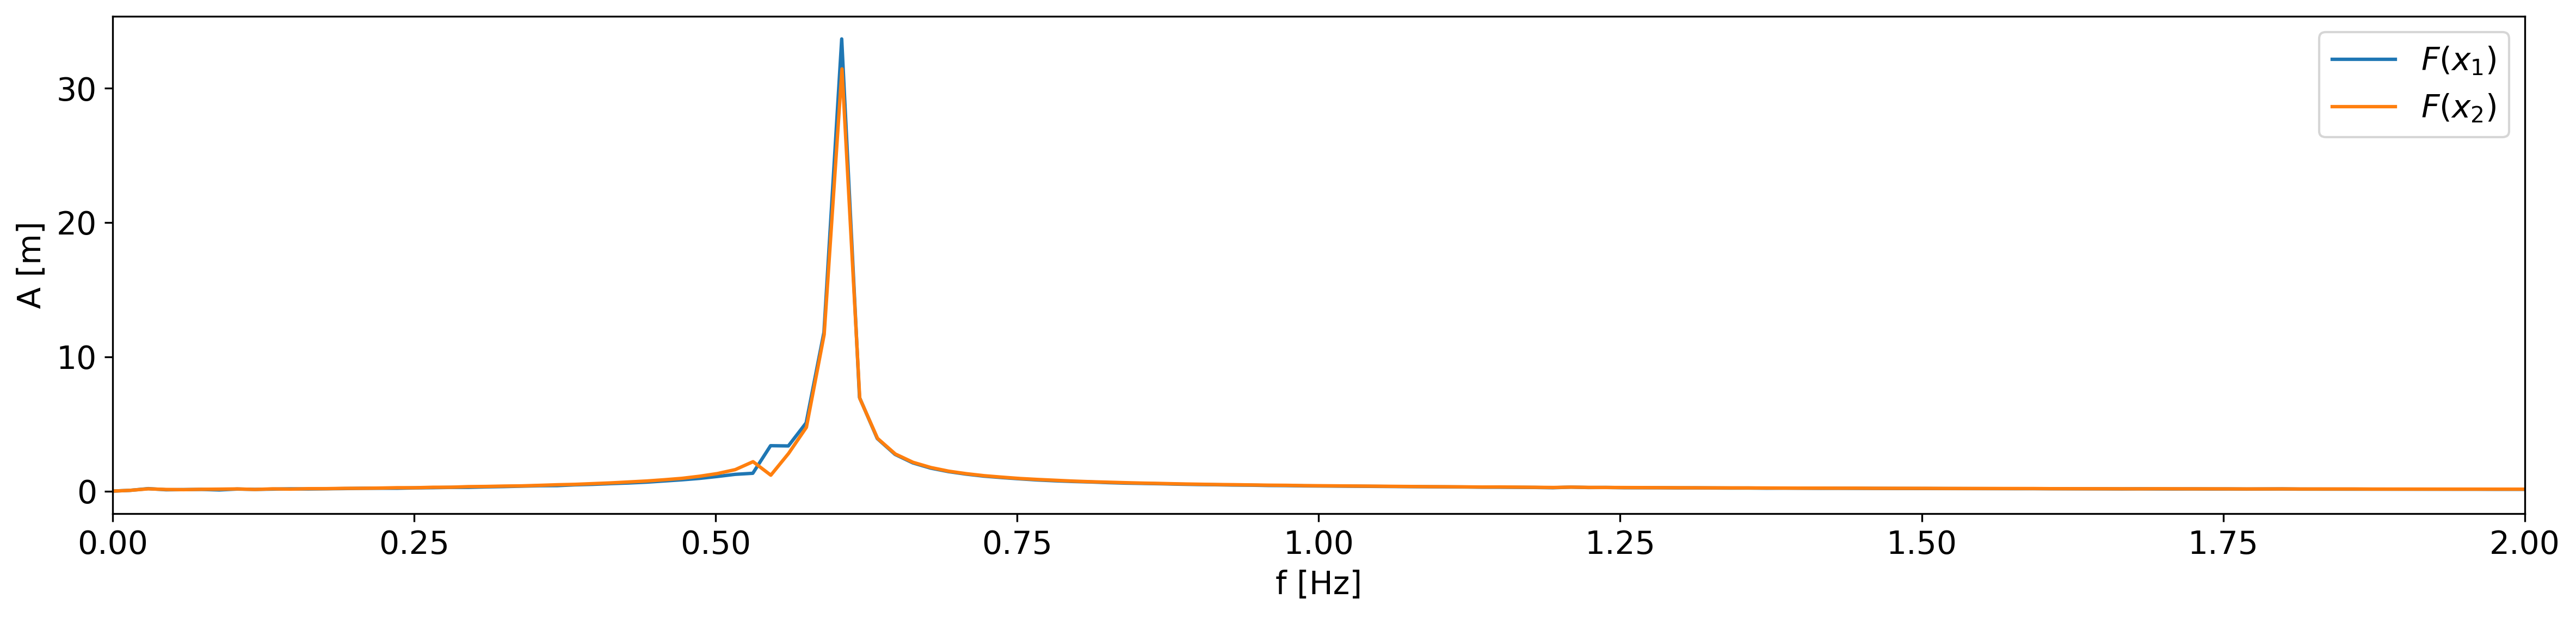
\includegraphics[width=\linewidth]{counterphase_1_fft}
    \caption{Wykres transformaty fouriera dla danych z wykresu \ref{fig:beats_0}}
    \label{fig:coutner_phase_0_fft}
\end{figure}
Uzyskujemy w ten sposób dwie częstotliwości
\[
    f_{d_10} = (0{,}536 \pm 0{,}016) \, Hz ,\quad f_{d_11} = (0{,}598 \pm 0{,}016) \, Hz
\]

To samo wykonujemy dla \(d = (40 \pm 0{,}1) cm\)
\begin{figure}[H]
    \centering
    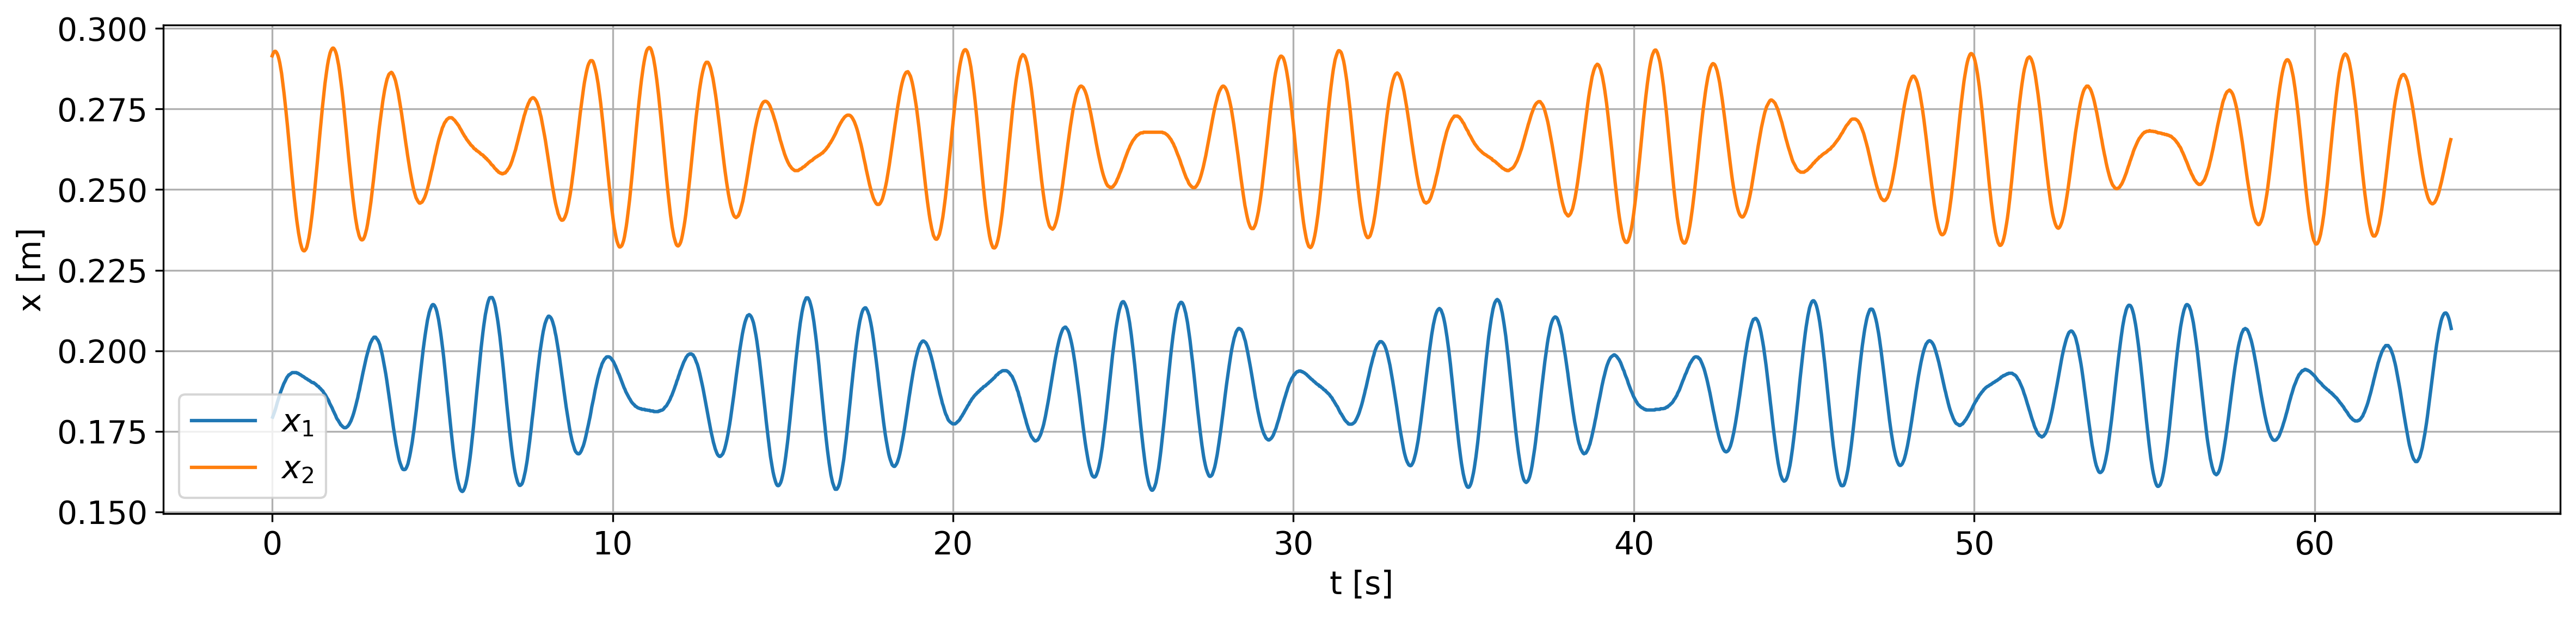
\includegraphics[width=\linewidth]{beats_2}
    \caption{Wykres zależności wychlenia wachadła lewego \(x_1\) i prawego \(x_2\) od czasu \(t\), dla wachadeł dudniących}
    \label{fig:beats_1}
\end{figure}
\begin{figure}[H]
    \centering
    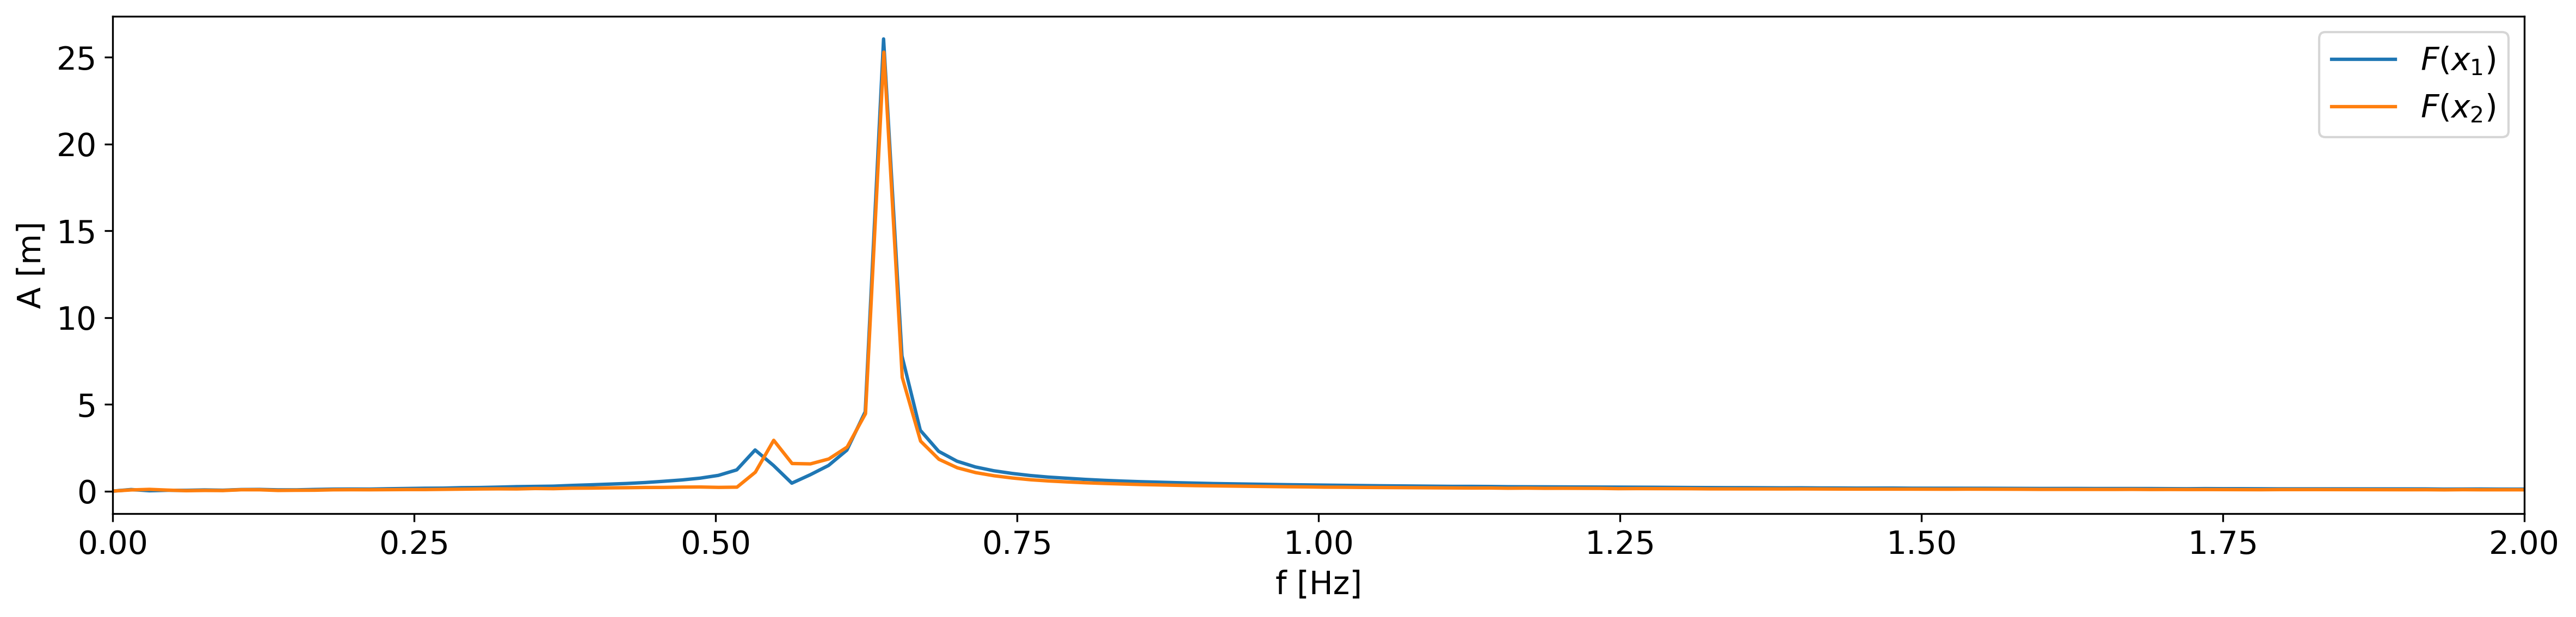
\includegraphics[width=\linewidth]{counterphase_2_fft}
    \caption{Wykres transformaty fouriera dla danych z wykresu \ref{fig:beats_1}}
    \label{fig:coutner_phase_1_fft}
\end{figure}
Uzyskujemy w ten sposób dwie częstotliwości
\[
    f_{d_20} = (0{,}547 \pm 0{,}016) \, Hz ,\quad f_{d_21} = (0{,}641 \pm 0{,}016) \, Hz
\]

Finalnie dla \(d = (45 \pm 0{,}1) cm\)
\begin{figure}[H]
    \centering
    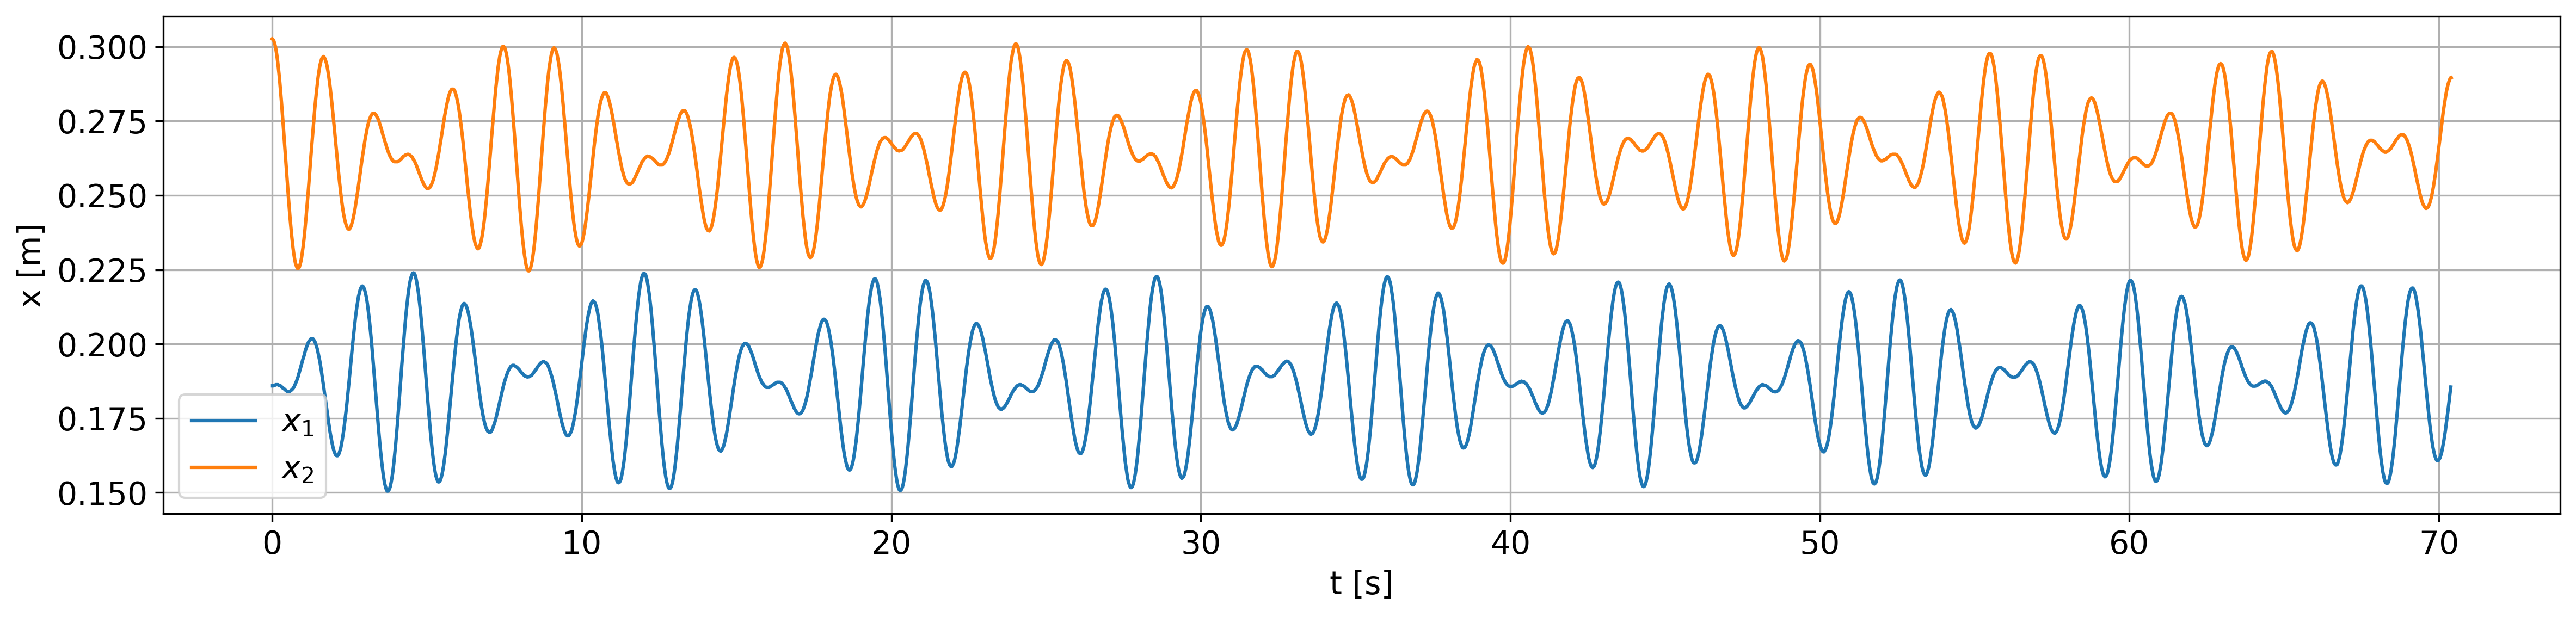
\includegraphics[width=\linewidth]{beats_3}
    \caption{Wykres zależności wychlenia wachadła lewego \(x_1\) i prawego \(x_2\) od czasu \(t\), dla wachadeł dudniących}
    \label{fig:beats_2}
\end{figure}
\begin{figure}[H]
    \centering
    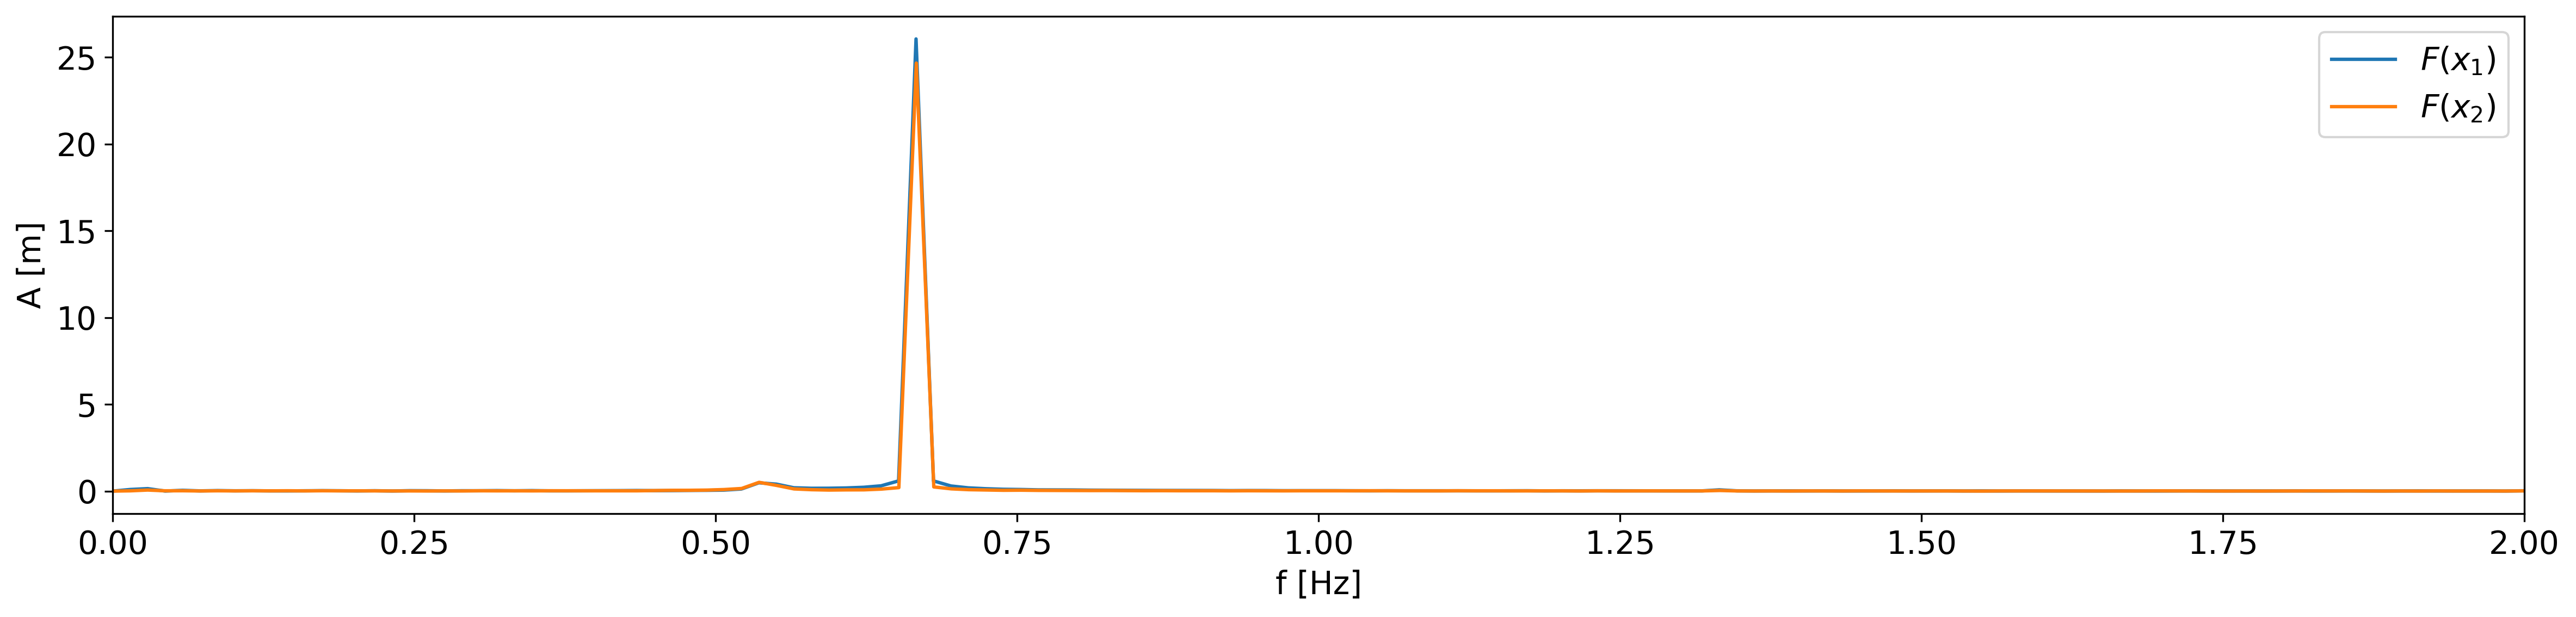
\includegraphics[width=\linewidth]{counterphase_3_fft}
    \caption{Wykres transformaty fouriera dla danych z wykresu \ref{fig:beats_2}}
    \label{fig:coutner_phase_2_fft}
\end{figure}
Uzyskujemy w ten sposób dwie częstotliwości
\[
    f_{d_30} = (0{,}540 \pm 0{,}015) \, Hz ,\quad f_{d_31} = (0{,}668 \pm 0{,}015) \, Hz
\]
\section{Podsumowanie}



\newpage

\begin{thebibliography}{2}

\bibitem{skrypt}
\emph{Wachadła sprzężone}, Aneta Drabińska, Roman J. Nowak i Andrzej Witowski, Uniwersytet Warszawski.

\end{thebibliography}

\end{document}
